\documentclass[UTF8,11pt]{ctexart}

\usepackage[a4paper,margin=1in]{geometry}
\usepackage{amsmath,amssymb,mathtools,bm}
\usepackage{booktabs,tabularx,array}
\usepackage{enumitem}
\usepackage[hidelinks]{hyperref}
\usepackage{xcolor}
\usepackage{graphicx}
\makeatletter
\setlength{\@fptop}{0pt}
\makeatother

\newcommand{\E}{\mathbb{E}}
\newcommand{\R}{\mathbb{R}}
\newcommand{\cH}{\mathcal{H}}
\newcommand{\cF}{\mathcal{F}}
\newcommand{\cL}{\mathcal{L}}
\newcommand{\Law}{\operatorname{Law}}
\newcommand{\MMD}{\operatorname{MMD}}
\newcommand{\dd}{\,\mathrm d}
\newcolumntype{Y}{>{\raggedright\arraybackslash}X}

\title{Weak Bridge Velocity Matching\\
\large 从点态条件速度估计到弱形式桥流量对齐}
\author{}
\date{\today}

\begin{document}

\maketitle

\section{已有方法简述：从 MAGT 到随机插值速度版本}

MAGT 的出发点是把生成问题压缩到一个固定插值层级上。给定真实数据端点
\[
X_1\sim p_{\rm data},
\]
以及一步生成器
\[
h_\theta:\R^d\to\R^D,
\qquad
U\sim\pi,
\qquad
x_{\rm gen}=h_\theta(U),
\]
固定层级的平滑数据和模型平滑分布可以写成
\[
Y_\tau^d=\alpha_\tau X_1+\sigma_\tau\varepsilon,
\qquad
Y_{\theta,\tau}=\alpha_\tau h_\theta(U)+\sigma_\tau\varepsilon,
\qquad
\varepsilon\sim\mathcal N(0,I_D).
\]
因此 MAGT 类方法的核心可以理解为：在固定 \(\tau\) 上学习一个低维到高维的 one-step transport，使模型诱导的平滑分布接近数据平滑分布。这个设计保留了一步生成
\[
u\sim\pi,\qquad x_{\rm gen}=h_\theta(u),
\]
同时用固定层级的 denoising / score 信号降低直接匹配高维数据分布的难度。

从模型侧看，\(Y_{\theta,\tau}\) 的边缘密度是由 latent \(U\) 混合出来的 Gaussian mixture：
\[
p_{\theta,\tau}(y)
=
\int
\phi\left(y;\alpha_\tau h_\theta(u),\sigma_\tau^2 I_D\right)\pi(u)\,du .
\]
对 \(\log p_{\theta,\tau}(y)\) 求梯度，并把每个 mixture component 的 Gaussian score 对 posterior
\(U\mid Y_{\theta,\tau}=y\) 取平均，得到
\[
\begin{aligned}
\nabla_y\log p_{\theta,\tau}(y)
&=
\E_\theta\!\left[
\nabla_y\log \phi\left(y;\alpha_\tau h_\theta(U),\sigma_\tau^2 I_D\right)
\mid Y_{\theta,\tau}=y
\right]\\
&=
\frac{1}{\sigma_\tau^2}
\left(
\alpha_\tau
\E_\theta[h_\theta(U)\mid Y_{\theta,\tau}=y]
-y
\right).
\end{aligned}
\]
因此模型 score 的关键不在于额外学习一个新的函数，而在于如何估计 posterior mean
\[
m_{\theta,\tau}(y)=\E_\theta[h_\theta(U)\mid Y_{\theta,\tau}=y].
\]

需要注意的是，\(Y_\tau^d\) 和 \(Y_{\theta,\tau}\) 是两条不同平滑分布的随机变量。下面的
\(\widetilde s_{\theta,K,\tau}(y)\) 不是在一个固定的模型样本
\(Y_{\theta,\tau}\) 上定义的数值，而是模型诱导平滑密度在任意查询点 \(y\) 上的 score estimator。
训练时会把这个函数评估在真实数据桥的 noisy sample 上。

具体地，给定 anchors \(u_k\sim\tilde\pi(\cdot\mid y)\)，MAGT 用自归一化重要性采样近似 posterior mean：
\[
\omega_k(y)
\propto
\frac{\pi(u_k)}{\tilde\pi(u_k\mid y)}
\phi\left(
y;\alpha_\tau h_\theta(u_k),\sigma_\tau^2 I_D
\right),
\qquad
w_k(y)=
\frac{\omega_k(y)}{\sum_{\ell=1}^K\omega_\ell(y)},
\]
\[
\widetilde m_{\theta,K,\tau}(y)
=
\sum_{k=1}^K w_k(y)h_\theta(u_k).
\]
对应的 transport-based score estimator 为
\[
\widetilde s_{\theta,K,\tau}(y)
=
\frac{
\alpha_\tau \widetilde m_{\theta,K,\tau}(y)-y
}{\sigma_\tau^2}.
\]
对训练样本 \(x_1^i\sim p_{\rm data}\)，采样
\[
y_{\tau,d}^i=\alpha_\tau x_1^i+\sigma_\tau\varepsilon^i,
\qquad
\varepsilon^i\sim\mathcal N(0,I_D).
\]
高斯条件 score 是
\[
s_{\rm cond}(y_{\tau,d}^i,x_1^i)
=
\nabla_{y_\tau}\log p(y_{\tau,d}^i\mid x_1^i)
=
\frac{\alpha_\tau x_1^i-y_{\tau,d}^i}{\sigma_\tau^2}.
\]
于是 MAGT 的固定层级 denoising score matching loss 为
\[
\ell_{\rm MAGT}(y_{\tau,d}^i,x_1^i;\theta)
=
\left\|
\widetilde s_{\theta,K,\tau}(y_{\tau,d}^i)
-
s_{\rm cond}(y_{\tau,d}^i,x_1^i)
\right\|_2^2,
\]
代入两个 score 的表达式，\(y_{\tau,d}^i\) 项相消，得到完全等价的后验均值预测形式：
\[
\ell_{\rm MAGT}(y_{\tau,d}^i,x_1^i;\theta)
=
\frac{\alpha_\tau^2}{\sigma_\tau^4}
\left\|
\widetilde m_{\theta,K,\tau}(y_{\tau,d}^i)-x_1^i
\right\|_2^2.
\]
因此 MAGT 的训练可以直白理解为：在真实数据桥的 noisy query point
\(y_{\tau,d}^i\) 上，用模型 posterior mean estimator
\(\widetilde m_{\theta,K,\tau}\) 去预测干净数据端点 \(x_1^i\)。
\[
L_{n,K}^{\rm MAGT}(\theta)
=
\frac1n
\sum_{i=1}^n
\ell_{\rm MAGT}(y_{\tau,d}^i,x_1^i;\theta).
\]
随机插值速度版本在这个基础上换成 velocity matching 语言。真实线性桥为
\[
X_\tau^d=(1-\tau)X_0+\tau X_1,
\qquad
V^d=X_1-X_0,
\]
模型桥为
\[
X_{\theta,\tau}=(1-\tau)X_0+\tau h_\theta(U),
\qquad
V^\theta=h_\theta(U)-X_0.
\]
模型不再学习自由速度网络，而是使用由生成端点诱导的 projected velocity：
\[
v_{\theta,\tau}(x_\tau)
=
\E_\theta[h_\theta(U)-X_0\mid X_{\theta,\tau}=x_\tau].
\]
随机插值速度版本的基本 velocity loss 是
\[
\mathcal L_{\rm SI\text{-}VM}(\theta)
=
\E\left[
\left\|
v_{\theta,\tau}(X_\tau^d)
-
(X_1-X_0)
\right\|_2^2
\right].
\]
这里和 MAGT 的训练点用法一致：\(X_\tau^d\) 是从真实数据桥采到的 query point；
\(v_{\theta,\tau}(\cdot)\) 是模型桥诱导出的条件速度函数，只是被评估在数据桥的 query point 上。
在线性无噪声插值下，给定 \(x_\tau\) 和 anchor \(u\) 可以反推出
\[
X_0
=
\frac{x_\tau-\tau h_\theta(u)}{1-\tau}.
\]
于是令
\[
m_{\theta,\tau}(x_\tau)
:=
\E_\theta[h_\theta(U)\mid X_{\theta,\tau}=x_\tau],
\]
就有
\[
v_{\theta,\tau}(x_\tau)
=
\frac{
m_{\theta,\tau}(x_\tau)-x_\tau
}{1-\tau}.
\]
同时，在数据桥上有
\[
V^d=X_1-X_0=\frac{X_1-X_\tau^d}{1-\tau}.
\]
所以 velocity loss 也可以化成后验均值预测形式：
\[
\mathcal L_{\rm SI\text{-}VM}(\theta)
=
\frac{1}{(1-\tau)^2}
\E\left[
\left\|
m_{\theta,\tau}(X_\tau^d)-X_1
\right\|_2^2
\right].
\]
如果使用有限 anchors 近似 \(m_{\theta,\tau}\)，则训练样本级别就是
\[
\ell_{\rm SI\text{-}VM}(x_{\tau,d}^i,x_1^i;\theta)
=
\frac{1}{(1-\tau)^2}
\left\|
\widehat m_{\theta,K,\tau}(x_{\tau,d}^i)-x_1^i
\right\|_2^2.
\]
因此线性随机插值速度版本和 MAGT 在形式上非常接近：都在数据桥的 query point 上，用模型诱导的 endpoint posterior mean 去预测真实数据端点。WBVM 则进一步改换监督对象：
不再估计点态条件速度或后验均值，而是直接比较生成器诱导桥与数据桥的弱流量。

\clearpage

\section{两个固定层级 loss 的后验均值形式}

去掉一般随机插值以后，MAGT 和线性随机插值速度版可以放在同一个模板下看：训练输入都来自数据桥，模型提供一个 endpoint posterior mean estimator，目标都是预测真实数据端点。

\paragraph{MAGT。}
数据 query point 是
\[
y_{\tau,d}=\alpha_\tau x_1+\sigma_\tau\varepsilon.
\]
模型给出 posterior mean estimator
\[
\widetilde m_{\theta,K,\tau}(y)
\approx
\E_\theta[h_\theta(U)\mid Y_{\theta,\tau}=y].
\]
原本的 score matching loss 等价于
\[
\ell_{\rm MAGT}(y_{\tau,d},x_1;\theta)
=
\frac{\alpha_\tau^2}{\sigma_\tau^4}
\left\|
\widetilde m_{\theta,K,\tau}(y_{\tau,d})-x_1
\right\|_2^2.
\]
所以 MAGT 本质上是在 noisy data query 上预测 clean endpoint。

\paragraph{线性随机插值速度版。}
数据 query point 是
\[
x_{\tau,d}=(1-\tau)x_0+\tau x_1.
\]
模型桥的 endpoint posterior mean 为
\[
m_{\theta,\tau}(x)
=
\E_\theta[h_\theta(U)\mid X_{\theta,\tau}=x].
\]
由于
\[
v_{\theta,\tau}(x)=\frac{m_{\theta,\tau}(x)-x}{1-\tau},
\qquad
V^d=\frac{x_1-x_{\tau,d}}{1-\tau},
\]
velocity matching loss 等价于
\[
\ell_{\rm SI\text{-}VM}(x_{\tau,d},x_1;\theta)
=
\frac{1}{(1-\tau)^2}
\left\|
m_{\theta,\tau}(x_{\tau,d})-x_1
\right\|_2^2.
\]
如果用有限 anchors 近似 \(m_{\theta,\tau}\)，只需把上式中的 \(m_{\theta,\tau}\) 换成
\(\widehat m_{\theta,K,\tau}\)。

因此这两个固定层级版本的共同核心是
\[
\boxed{
\text{model endpoint posterior mean at data-bridge query}
\approx
\text{true data endpoint}.
}
\]
差别主要在桥的定义和比例常数：MAGT 的常数是 \(\alpha_\tau^2/\sigma_\tau^4\)，线性随机插值速度版的常数是 \((1-\tau)^{-2}\)。

\section{MAGT 第 3 部分的理论脉络}

MAGT 第 3 部分要证明的是一个固定层级理论：如果一步生成器
\[
\widetilde Y_0=\hat h_\lambda(U)
\]
在某个 Gaussian smoothing level \(t\) 上把 smoothed score 或 posterior mean 学准，那么未加噪的一步生成分布
\[
P_{\widetilde Y_0}
\]
也会在 \(W_2\) 意义下接近真实数据分布 \(P_{Y_0}\)。它的 bound 推导不是从训练误差一步跳到 endpoint error，而是经过下面的链条：
\[
\text{fixed-level score risk}
\Longrightarrow
\text{Fisher mismatch}
\Longrightarrow
\text{smoothed-level } W_2
\Longrightarrow
\text{endpoint } W_2 .
\]
其中最后一箭头是最有 MAGT 特色的 single-level pull-back：只用一个固定噪声层级，而不是像扩散模型那样沿全时间积分 score error。

\paragraph{关键定理一：single-level pull-back bound。}
令
\[
Y_t=\alpha_tY_0+\sigma_tZ,
\qquad
\widetilde Y_t=\alpha_t\widetilde Y_0+\sigma_tZ,
\qquad
\alpha_t=\sqrt{1-t},\quad \sigma_t^2=t.
\]
定义 denoiser mismatch
\[
E_{\rm MAG}(t)
=
\E_{Y\sim p_t}
\|m_{p,t}(Y)-m_{\tilde p,t}(Y)\|_2^2,
\]
其中
\[
m_{p,t}(y)=\E[Y_0\mid Y_t=y],
\qquad
m_{\tilde p,t}(y)=\E[\widetilde Y_0\mid \widetilde Y_t=y].
\]
Tweedie 公式给出
\[
E_{\rm MAG}(t)
=
\frac{t^2}{1-t}\,
\E_{Y\sim p_t}
\|\nabla\log p_t(Y)-\nabla\log\tilde p_t(Y)\|_2^2.
\]
因此 posterior mean error 等价于 fixed-level Fisher error。MAGT 的 pull-back 定理说明，在正则 transport、positive reach、latent LSI 和 tube regime 下，
\[
W_2(P_{Y_0},P_{\widetilde Y_0})
\le
C_{\rm PB}(t)\sqrt{E_{\rm MAG}(t)}.
\]
常数 \(C_{\rm PB}(t)\) 来自三部分：平滑层的 LSI--Fisher 到 \(W_2\) 控制、VP probability flow 的稳定性，以及流形管状邻域中的 Hessian bound。小噪声时主导尺度为
\[
C_{\rm PB}(t)=O(t^{-1}),
\]
所以 \(t\) 不能无脑取很小：小 \(t\) 偏差小，但 posterior 更尖、MC 方差和 pull-back 常数更差。

\paragraph{关键定理二：score-matching excess-risk bound。}
理想无限 anchor 风险写作
\[
R(h)=
\E\left[
\|s_t(Y_t;h)-\nabla_{Y_t}\log p(Y_t\mid Y_0)\|_2^2
\right].
\]
条件 score 的无偏性给出正交分解：
\[
R(h)-R(h^*)
=
\E_{Y\sim p_t}
\|\nabla\log p_t^h(Y)-\nabla\log p_t(Y)\|_2^2.
\]
也就是说，population score-matching excess risk 正好校准到 Fisher mismatch。随后用 bracketing entropy 控制经验风险最小化器；若 finite-anchor loss 与理想 loss 的统一扰动足够小，且 entropy integral 满足相应条件，则
\[
\Pr\{\rho(h^*,\hat h_\lambda)\ge \varepsilon\}
\le
4\exp(-c_en\varepsilon^2),
\]
其中
\[
\rho^2(h^*,h)=R(h)-R(h^*).
\]
这一部分本质上是 \(M\)-estimator 经验过程模板：正交分解负责校准目标，finite-anchor perturbation 负责把实际训练 loss 接回理想 loss。

\paragraph{关键定理三：finite-sample generation fidelity。}
把 pull-back bound、excess-risk bound、ReLU 逼近误差和 anchor 近似误差合并，得到
\[
\begin{aligned}
\E W_2(P_{Y_0},P_{\widetilde Y_0})
\le C_{\rm PB}(t)\Bigg[
&c_1(WL)^{-\frac{2(\eta+1)}{d^*}}
+c_2\sigma_t^{-(\eta+2)}
\left(
\frac{(WL)^2\log^5(WL)}{n}
\right)^{\frac{\eta+1}{2\eta}}\\
&+c_3\varepsilon(\tilde\pi,t,K)
\Bigg].
\end{aligned}
\]
前三项分别对应神经网络逼近、统计估计、有限 anchors / 重要性采样误差。平衡宽深乘积 \(WL\) 后，主率为
\[
\left(\frac{n}{\log^5 n}\right)^{-\frac{\eta+1}{2\eta+d^*}}
\]
外加 anchor error。这里最重要的叙事点是 rate 依赖 intrinsic dimension \(d^*\)，而不是 ambient dimension \(D\)。

\paragraph{证明结构的压缩版。}
整个 bound 可以记成四句：
\begin{enumerate}[leftmargin=2em]
\item Tweedie：posterior mean error \(\Longleftrightarrow\) score / Fisher error。
\item LSI：fixed-level Fisher error \(\Longrightarrow\) smoothed \(W_2\)。
\item VP pull-back：smoothed \(W_2\) 和 score-gap growth \(\Longrightarrow\) endpoint \(W_2\)。
\item Empirical process：经验 score matching \(\Longrightarrow\) Fisher risk rate，再加 finite-anchor perturbation。
\end{enumerate}

\section{两条桥}

真实数据桥为
\[
X_\tau^d=(1-\tau)X_0+\tau X_1,
\qquad
V^d=X_1-X_0.
\]
生成器诱导桥为
\[
X_{\theta,\tau}=(1-\tau)X_0+\tau h_\theta(U),
\qquad
V^\theta=h_\theta(U)-X_0.
\]
其中 \(X_0\sim p_0\)、\(X_1\sim p_{\rm data}\)、\(U\sim\pi\)。最终生成仍然是一步：
\[
u\sim\pi,\qquad x_{\rm gen}=h_\theta(u).
\]

如果走点态速度路线，就会定义 Markovian projected velocities：
\[
v_{d,\tau}(x)=\E[V^d\mid X_\tau^d=x],
\qquad
v_{\theta,\tau}(x)=\E[V^\theta\mid X_{\theta,\tau}=x].
\]
WBVM 刻意避开对 \(v_{\theta,\tau}\) 的显式估计。

\section{弱连续性方程}

设 \(\rho_\tau^d=\Law(X_\tau^d)\)，\(\rho_{\theta,\tau}=\Law(X_{\theta,\tau})\)。形式上，概率流满足连续性方程
\[
\partial_\tau \rho_\tau+\operatorname{div}(\rho_\tau v_\tau)=0.
\]
对任意光滑测试函数 \(\varphi:\R^D\to\R\)，弱形式为
\[
\frac{\dd}{\dd\tau}\E[\varphi(X_\tau)]
=
\E[\nabla\varphi(X_\tau)^\top V].
\]
因此定义弱桥流量差异：
\[
\Delta_\theta(\varphi,\tau)
=
\E[\nabla\varphi(X_{\theta,\tau})^\top V^\theta]
-
\E[\nabla\varphi(X_\tau^d)^\top V^d].
\]
主目标可以只保留弱桥流量差异。这里必须把测试函数大小固定住。否则由于
\(\Delta_\theta(c\varphi,\tau)=c\Delta_\theta(\varphi,\tau)\)，无约束的
\(\sup_{\varphi\in\cF}|\Delta_\theta(\varphi,\tau)|^2\) 会退化成 \(0\) 或 \(\infty\)。
因此令 \((\cF,\|\cdot\|_{\cF})\) 为带范数的测试函数空间，定义
\[
D_{\rm flux}^2(\theta,\tau)
=
\sup_{\varphi\in\cF,\ \|\varphi\|_{\cF}\le 1}
\left|
\Delta_\theta(\varphi,\tau)
\right|^2.
\]
对应的 all-time 损失函数为
\[
\cL_{\rm WBVM}^{\rm all}(\theta)
=
\int_0^1
D_{\rm flux}^2(\theta,\tau)
\dd\tau.
\]

\section{两种训练模式}

\paragraph{模式一：all-time pure flux matching。}
如果训练时对 \(\tau\sim{\rm Unif}[0,1]\) 采样，并且同一个 \(h_\theta\) 被所有时间层级共享，那么随机训练目标就是在近似
\[
\cL_{\rm WBVM}^{\rm all}(\theta)
=
\int_0^1 D_{\rm flux}^2(\theta,\tau)\dd\tau.
\]
在 population 层面，如果测试函数类足够丰富，并且
\[
D_{\rm flux}^2(\theta,\tau)=0,\qquad \forall \tau\in[0,1],
\]
并且两条桥有相同初始分布，那么可以由连续性方程推出
\[
h_\theta(U)\overset d=X_1.
\]
这是 WBVM 最干净的理论版本。

\paragraph{模式二：validation-selected single-level WBVM。}
如果希望采用固定层级，则不要声称单个 \(\tau\) 的 flux loss 本身足够识别 endpoint。更稳妥的做法是把 \(\tau\) 当作候选桥层级：
\[
\mathcal T=\{\tau_1,\ldots,\tau_m\}.
\]
对每个 \(\tau\in\mathcal T\) 单独训练候选生成器
\[
\hat\theta_\tau
=
\arg\min_\theta
D_{\rm flux}^2(\theta,\tau).
\]
然后用验证集在 endpoint 上选层级：
\[
\tau^\star
=
\arg\min_{\tau\in\mathcal T}
\widehat D_{\rm val}
\left(
P_{h_{\hat\theta_\tau}(U)},P_{\rm val}
\right).
\]
最终生成器为
\[
x_{\rm gen}=h_{\hat\theta_{\tau^\star}}(u),
\qquad u\sim\pi.
\]
这个版本的逻辑是：single-level flux loss 负责产生候选 \(h_{\hat\theta_\tau}\)，endpoint validation 负责选择最接近 \(X_1\) 的候选。

\section{三种实现路线总览}

\begin{center}
{\small
\begin{tabularx}{\linewidth}{@{}p{0.18\linewidth}YYY@{}}
\toprule
路线 & 核心对象 & 优点 & 风险 \\
\midrule
RKHS 核方法 & 闭式 weak flux discrepancy & 无 neural critic，理论最干净 & \(O(B^2)\)，带宽敏感，kernel Hessian 噪声 \\
Vector-flux MMD & vector flux measure & 实现直接，可做 flux-only baseline & 可能惩罚 divergence-free 的流量差异 \\
Sobolev critic & 学习测试函数，近似 \(H^{-1}\) 残差 & 最接近 PDE 弱形式，可扩展 & 对抗训练和高阶自动微分成本 \\
\bottomrule
\end{tabularx}
}
\end{center}

推荐推进顺序：
\[
\boxed{
\text{RKHS derivative-kernel}
\rightarrow
\text{vector-flux MMD}
\rightarrow
\text{Sobolev neural critic}
}
\]

\section{路线一：RKHS Derivative-Kernel WBVM}

令 \(\cH_k\) 是标量 RKHS，核为 \(k(x,x')\)。由导数再生性质，
\[
\partial_i\varphi(x)
=
\langle \varphi,\partial_{x_i}k(x,\cdot)\rangle_{\cH_k}.
\]
于是
\[
\nabla\varphi(x)^\top v
=
\left\langle
\varphi,
\sum_{i=1}^D v_i\partial_{x_i}k(x,\cdot)
\right\rangle_{\cH_k}.
\]
定义 flux mean embedding：
\[
\mu_{\theta,\tau}^{\rm flux}
=
\E\left[
\sum_{i=1}^D V_i^\theta
\partial_{x_i}k(X_{\theta,\tau},\cdot)
\right],
\]
\[
\mu_{d,\tau}^{\rm flux}
=
\E\left[
\sum_{i=1}^D V_i^d
\partial_{x_i}k(X_\tau^d,\cdot)
\right].
\]
则
\[
\Delta_\theta(\varphi,\tau)
=
\left\langle
\varphi,
\mu_{\theta,\tau}^{\rm flux}
-
\mu_{d,\tau}^{\rm flux}
\right\rangle_{\cH_k}.
\]
因此 RKHS 版本就是取
\[
\cF=\cH_k,
\qquad
\|\varphi\|_{\cF}=\|\varphi\|_{\cH_k}.
\]
在 RKHS 单位球上取上确界，得到闭式 discrepancy：
\[
D_{\rm RKHS\text{-}flux}^2(\theta,\tau)
=
\sup_{\|\varphi\|_{\cH_k}\le 1}
\left|
\Delta_\theta(\varphi,\tau)
\right|^2
=
\left\|
\mu_{\theta,\tau}^{\rm flux}
-
\mu_{d,\tau}^{\rm flux}
\right\|_{\cH_k}^2.
\]
这里的等号来自 Cauchy--Schwarz 和 Riesz 表示定理：\(\mu_{\theta,\tau}^{\rm flux}-\mu_{d,\tau}^{\rm flux}\) 正是线性泛函 \(\Delta_\theta(\cdot,\tau)\) 在 RKHS 中的 representer。

经验估计时应显式区分模型桥样本量和数据桥样本量。记
\[
\{(x_i^\theta,v_i^\theta)\}_{i=1}^{n_\theta},
\qquad
\{(x_j^d,v_j^d)\}_{j=1}^{n_d},
\qquad
H_k(x,x')=\nabla_x\nabla_{x'}k(x,x').
\]
对 RBF 核
\[
k_\sigma(x,x')
=
\exp\left(-\frac{\|x-x'\|^2}{2\sigma^2}\right),
\]
有
\[
\nabla_x\nabla_{x'}k_\sigma(x,x')
=
k_\sigma(x,x')
\left[
\frac{I_D}{\sigma^2}
-
\frac{(x-x')(x-x')^\top}{\sigma^4}
\right].
\]
特别地，当 \(x=x'\) 时，
\[
H_{k_\sigma}(x,x)=\frac{I_D}{\sigma^2},
\qquad
v^\top H_{k_\sigma}(x,x)v
=
\frac{\|v\|^2}{\sigma^2}.
\]
所以同组对角项会把速度范数直接带入目标。为避免 loss 被 \(\|v\|^2/\sigma^2\) 主导，经验估计直接采用去掉同组对角项的 U-statistic：
\[
\begin{aligned}
\widehat D_{\rm RKHS\text{-}flux,U}^2
&=
\frac{1}{n_\theta(n_\theta-1)}
\sum_{i\ne i'}
(v_i^\theta)^\top
H_k(x_i^\theta,x_{i'}^\theta)
v_{i'}^\theta
\\
&\quad+
\frac{1}{n_d(n_d-1)}
\sum_{j\ne j'}
(v_j^d)^\top
H_k(x_j^d,x_{j'}^d)
v_{j'}^d
\\
&\quad-
\frac{2}{n_\theta n_d}
\sum_{i=1}^{n_\theta}\sum_{j=1}^{n_d}
(v_i^\theta)^\top
H_k(x_i^\theta,x_j^d)
v_j^d .
\end{aligned}
\]
这个修改只去掉模型--模型和数据--数据内部的 \(i=i'\)、\(j=j'\) 项；模型--数据交叉项不需要去对角，因为它们来自两组样本。

\section{路线二：Vector-Flux MMD WBVM}

路线一的 RKHS-flux 是从弱连续性方程出发：
\[
\Delta_\theta(\varphi,\tau)
=
\E[\nabla\varphi(X_{\theta,\tau})^\top V^\theta]
-
\E[\nabla\varphi(X_\tau^d)^\top V^d].
\]
也就是说，它只用形如
\[
g(x)=\nabla\varphi(x)
\]
的测试向量场去观察流量差异。路线二换一个更直接的角度：不先取散度，也不限制测试向量场必须是某个标量函数的梯度，而是直接把
\[
\rho(x)v(x)
\]
看作一个向量值测度，并在向量值 RKHS 中做 MMD。

具体地，定义两条桥在层级 \(\tau\) 的 vector flux measure：
\[
F_{\theta,\tau}=\rho_{\theta,\tau}(x)v_{\theta,\tau}(x),
\qquad
F_{d,\tau}=\rho_\tau^d(x)v_{d,\tau}(x).
\]
在采样形式下，它们分别由
\[
(X_{\theta,\tau},V^\theta),
\qquad
(X_\tau^d,V^d)
\]
给出，其中
\[
X_{\theta,\tau}=(1-\tau)X_0+\tau h_\theta(U),
\qquad
V^\theta=h_\theta(U)-X_0,
\]
\[
X_\tau^d=(1-\tau)X_0+\tau X_1,
\qquad
V^d=X_1-X_0.
\]
如果采用速度归一化版本，则把上式中的 \(V^\theta,V^d\) 替换为
\(\widetilde V^\theta,\widetilde V^d\)。这时目标应理解为 normalized flux discrepancy，而不是原始物理速度的精确 flux。

取一个标量核 \(k\)，构造矩阵值核
\[
K(x,x')=k(x,x')I_D
\]
及其向量值 RKHS
\[
\cH_K\simeq \cH_k^D .
\]
路线二的目标可以写成一个向量测试函数的 dual norm：
\[
D_{\rm vMMD}(\theta,\tau)
=
\sup_{\|g\|_{\cH_K}\le 1}
\left|
\E[g(X_{\theta,\tau})^\top V^\theta]
-
\E[g(X_\tau^d)^\top V^d]
\right|.
\]
由 RKHS 的 reproducing property，这个 supremum 等价于两个 vector flux mean embeddings 的距离：
\[
D_{\rm vMMD}^2(\theta,\tau)
=
\left\|
\E[k(X_{\theta,\tau},\cdot)V^\theta]
-
\E[k(X_\tau^d,\cdot)V^d]
\right\|_{\cH_K}^2.
\]
因此 population 闭式为
\[
\begin{aligned}
D_{\rm vMMD}^2
&=
\E[(V^\theta)^\top V^{\theta\prime}
k(X_{\theta,\tau},X_{\theta,\tau}')]
\\
&\quad+
\E[(V^d)^\top V^{d\prime}
k(X_\tau^d,X_\tau^{d\prime})]
\\
&\quad-
2\E[(V^\theta)^\top V^d
k(X_{\theta,\tau},X_\tau^d)].
\end{aligned}
\]

mini-batch 训练时，记模型桥样本为
\[
\{(x_i^\theta,v_i^\theta)\}_{i=1}^{n_\theta},
\]
数据桥样本为
\[
\{(x_j^d,v_j^d)\}_{j=1}^{n_d}.
\]
为了避免同组对角项
\[
k(x_i,x_i)\|v_i\|^2
\]
再次让速度范数主导 loss，经验估计建议使用 U-statistic：
\[
\begin{aligned}
\widehat D_{\rm vMMD,U}^2
&=
\frac{1}{n_\theta(n_\theta-1)}
\sum_{i\ne i'}
(v_i^\theta)^\top v_{i'}^\theta
k(x_i^\theta,x_{i'}^\theta)
\\
&\quad+
\frac{1}{n_d(n_d-1)}
\sum_{j\ne j'}
(v_j^d)^\top v_{j'}^d
k(x_j^d,x_{j'}^d)
\\
&\quad-
\frac{2}{n_\theta n_d}
\sum_{i=1}^{n_\theta}\sum_{j=1}^{n_d}
(v_i^\theta)^\top v_j^d
k(x_i^\theta,x_j^d).
\end{aligned}
\]
和路线一一样，数据--数据项不依赖 \(\theta\)，训练生成器时可以从反向传播图中去掉；但记录完整
\(\widehat D_{\rm vMMD,U}^2\) 作为 held-out diagnostic 更清楚。

对应的训练目标为
\[
\cL_{\rm vMMD\text{-}WBVM}
=
D_{\rm vMMD}^2(\theta,\tau).
\]

这条路线和路线一的关系可以用一句话概括：
\[
\boxed{
\text{路线一匹配 } \nabla\varphi \text{ 能看到的 flux；路线二匹配所有 RKHS vector field 能看到的 flux。}
}
\]
因此路线二通常是一个更强的条件。如果 \(k\) 对有限 signed measure 足够 characteristic，
\[
D_{\rm vMMD}(\theta,\tau)=0
\]
会推出向量值测度意义下的
\[
F_{\theta,\tau}=F_{d,\tau}.
\]
这当然会推出两者散度相同；但连续性方程真正需要的只是
\[
\operatorname{div} F_{\theta,\tau}
=
\operatorname{div} F_{d,\tau}.
\]
所以路线二可能会额外惩罚一些
\[
\operatorname{div}(F_{\theta,\tau}-F_{d,\tau})=0
\]
但 \(F_{\theta,\tau}\ne F_{d,\tau}\) 的 divergence-free circulation 差异。这是它理论上比路线一更强、也更不精确贴合 PDE 弱形式的地方。

不过它有三个实际优点。第一，实现只需要普通 kernel Gram matrix 和速度内积，不需要计算
\[
\nabla_x\nabla_{x'}k(x,x')
\]
这样的 Hessian kernel。第二，它很适合作为 flux-only baseline，因为可以直接检查“位置相近且方向相近”的流量是否被对齐。第三，它很自然地扩展到 feature space。若使用一个特征映射
\[
Z=\psi(X),
\]
则 feature-space flux 速度可以写成
\[
\dot Z
=
J_\psi(X)V,
\]
于是只需把
\[
(x,v)
\]
替换为
\[
(\psi(x),J_\psi(x)v)
\]
再计算同一个 vector MMD。实际实现中，如果不想显式形成 Jacobian，也可以用有限差分近似
\[
J_\psi(X)V
\approx
\frac{\psi(X+\epsilon V)-\psi(X)}{\epsilon}.
\]
这给图像实验一个很清楚的升级方向：生成器仍然可以在 pixel 或 latent 中输出，但 flux discrepancy 在 LeNet、MAE 或其他语义特征空间中计算。

因此路线二适合承担一个偏工程和实验的角色：它不是最贴近连续性方程理论的版本，但它是最容易稳定实现、最容易搬到 feature space、也最适合快速验证“弱桥流量对齐是否真的给 endpoint 生成带来收益”的版本。

\section{路线三：Sobolev Neural-Critic WBVM}

Sobolev 版本直接保留弱形式，并学习测试函数。严格的 dual-norm 写法是先固定一个 Sobolev 单位球，例如
\[
D_{\rm Sob\text{-}flux}^2(\theta,\tau)
=
\sup_{\|\varphi\|_{\rm Sob}\le 1}
\left|
\Delta_\theta(\varphi,\tau)
\right|^2.
\]
实际训练中，更常用的是等价的正则化 critic 形式：
\[
D_{\rm Sob\text{-}flux}^2(\theta,\tau)
=
\sup_\varphi
\left\{
2\Delta_\theta(\varphi,\tau)
-
\E_{\bar\rho_\tau}\|\nabla\varphi(X)\|^2
-
\epsilon\E_{\bar\rho_\tau}|\varphi(X)|^2
\right\},
\]
其中
\[
\bar\rho_\tau
=
\frac12\rho_{\theta,\tau}
+
\frac12\rho_\tau^d.
\]
这里的梯度惩罚和 \(\epsilon\)-项正是在控制 critic 的 Sobolev 大小，避免无约束放大 \(\varphi\) 导致目标发散。
用神经网络 \(\varphi_\eta\) 实现时，critic 更新为
\[
\max_\eta
\left[
2\Delta_\theta(\varphi_\eta,\tau)
-
\E_{\bar\rho_\tau}\|\nabla\varphi_\eta(X)\|^2
-
\epsilon\E_{\bar\rho_\tau}|\varphi_\eta(X)|^2
\right].
\]
生成器更新为
\[
\min_\theta
D_{\rm Sob\text{-}flux}^2(\theta,\tau).
\]

这个目标近似一个 \(H^{-1}\) 型连续性方程残差：
\[
D_{\rm Sob\text{-}flux}(\theta,\tau)
\approx
\left\|
\operatorname{div}
(F_{\theta,\tau}-F_{d,\tau})
\right\|_{H^{-1}(\bar\rho_\tau)}.
\]
形式上，最优 critic 满足椭圆型弱问题：
\[
-
\operatorname{div}(\bar\rho_\tau\nabla\varphi^\star)
+
\epsilon\bar\rho_\tau\varphi^\star
=
-
\operatorname{div}(F_{\theta,\tau}-F_{d,\tau}).
\]

Sobolev critic 是最接近 PDE 理论的版本，但也是训练最难的版本。实际推进时可以加入速度归一化：
\[
V^\theta
\leftarrow
\frac{V^\theta}
{\operatorname{sg}(\sqrt{\E\|V^\theta\|^2}+\delta)},
\qquad
V^d
\leftarrow
\frac{V^d}
{\operatorname{sg}(\sqrt{\E\|V^d\|^2}+\delta)}.
\]

\section{理论命题}

\paragraph{命题一：all-time pure flux 的总体可识别性。}
假设两条桥有相同初始分布：
\[
X_{\theta,0}\overset d=X_0\overset d=X_0^d.
\]
如果对所有 \(\tau\in[0,1]\) 和所有 \(\varphi\in C_c^\infty(\R^D)\)，
\[
\E[\nabla\varphi(X_{\theta,\tau})^\top V^\theta]
=
\E[\nabla\varphi(X_\tau^d)^\top V^d],
\]
且对应连续性方程的弱解唯一，则
\[
\rho_{\theta,\tau}=\rho_\tau^d,\qquad \forall \tau\in[0,1].
\]
特别地，
\[
h_\theta(U)=X_{\theta,1}\overset d=X_1.
\]
这说明：如果所有时间层级的弱桥流量差异都为零，那么只保留 flux 项也足够推出 endpoint distribution 一致。

\paragraph{命题二：负 Sobolev 稳定性。}
对于合适的 Sobolev critic class，
\[
D_{\rm flux}(\theta,\tau)
\approx
\left\|
\operatorname{div}
(\rho_{\theta,\tau}v_{\theta,\tau}
-
\rho_\tau^d v_{d,\tau})
\right\|_{H^{-1}(\bar\rho_\tau)}.
\]
因此一个 all-time bound 应该类似于
\[
d_{\cH}(\rho_{\theta,1},\rho_1^d)
\le
C
\int_0^1
D_{\rm flux}(\theta,\tau)
\dd\tau.
\]

\paragraph{命题三：固定层级 pure flux 的限制。}
单个固定 \(\tau_0\) 的弱残差一般不能唯一确定 endpoint distribution。它最多约束
\[
\partial_\tau
(\rho_{\theta,\tau}-\rho_\tau^d)\big|_{\tau=\tau_0},
\]
不能推出
\[
\rho_{\theta,\tau_0}=\rho_{\tau_0}^d,
\qquad
\rho_{\theta,1}=\rho_1^d.
\]
因此 fixed-level WBVM 的理论表述应当是候选生成器训练，而不是完整可识别性定理。

\paragraph{命题四：候选验证选择的 oracle bound。}
令 \(\mathcal T\) 是有限候选集合，并对每个 \(\tau\in\mathcal T\) 得到候选模型
\[
\hat\theta_\tau
=
\arg\min_\theta
D_{\rm flux}^2(\theta,\tau).
\]
设真实 endpoint 距离为
\[
D(\tau)
=
D\left(P_{h_{\hat\theta_\tau}(U)},P_{X_1}\right),
\]
验证估计为 \(\widehat D_{\rm val}(\tau)\)。如果有一致收敛
\[
\sup_{\tau\in\mathcal T}
\left|
\widehat D_{\rm val}(\tau)-D(\tau)
\right|
\le
\epsilon_{\rm val},
\]
并且
\[
\tau^\star
=
\arg\min_{\tau\in\mathcal T}\widehat D_{\rm val}(\tau),
\]
则
\[
D(\tau^\star)
\le
\min_{\tau\in\mathcal T}D(\tau)
+
2\epsilon_{\rm val}.
\]
典型有限候选集合下，
\[
\epsilon_{\rm val}
=
O\left(
\sqrt{\frac{\log|\mathcal T|}{n_{\rm val}}}
\right)
\]
再加上生成样本的 Monte Carlo 误差。若候选集合中存在一个好层级 \(\bar\tau\)，使
\[
D(\bar\tau)\approx 0,
\]
则验证选择出的 \(h_{\hat\theta_{\tau^\star}}(U)\) 在 \(D\) 意义下接近 \(X_1\)。

\section{实验路线}

\paragraph{第一阶段：合成数据。}
用 2D moons、spiral、checkerboard，以及嵌入 \(D=50\) 或 \(D=100\) 的 helix / torus。核心目标不是刷新图像指标，而是验证：
\[
\text{weak flux signal 是否能稳定推动一步生成器学习。}
\]

\paragraph{第二阶段：all-time pure flux。}
训练同一个 \(h_\theta\)，每个 batch 随机采样
\[
\tau\sim{\rm Unif}[0.35,0.85],
\]
最小化
\[
\widehat{\cL}_{\rm WBVM}^{\rm all}
\approx
\frac1B\sum_{b=1}^B
\widehat D_{\rm RKHS\text{-}flux,U}^2(\theta,\tau_b).
\]
训练中使用共享 \(X_0\)、velocity RMS normalization 和固定多尺度 RBF 带宽；
评估 endpoint \(W_2\)、sliced \(W_2\)，以及 held-out weak flux residual。这个实验对应 all-time theory 的数值稳定版本。

\paragraph{第三阶段：validation-selected single-level。}
选候选集合
\[
\mathcal T=\{0.1,0.2,\ldots,0.9\}.
\]
分别训练
\[
\hat\theta_\tau
=
\arg\min_\theta \widehat D_{\rm RKHS\text{-}flux,U}^2(\theta,\tau),
\qquad \tau\in\mathcal T.
\]
每个候选训练 4000 steps。公共网络设置与 flow matching 基线保持一致：
5 层 ReLU MLP、width 512、AdamW 优化器和相同训练步数尺度。
然后用验证集 endpoint metric 选择
\[
\tau^\star
=
\arg\min_{\tau\in\mathcal T}
\widehat D_{\rm val}
\left(
P_{h_{\hat\theta_\tau}(U)},P_{\rm val}
\right).
\]
报告
\[
D_{\rm test}
\left(
P_{h_{\hat\theta_{\tau^\star}}(U)},P_{\rm test}
\right)
\]
以及 oracle gap
\[
D_{\rm test}(\tau^\star)
-
\min_{\tau\in\mathcal T}D_{\rm test}(\tau).
\]
这个实验对应候选验证选择理论，而不是单点 flux 可识别性理论。

\subsection{当前 RKHS-WBVM 模拟结果}

最新一版实验使用六个 Section 6.1 风格 toy 数据集：
rings2d、spiral2d、moons2d、checker2d、helix3d 和 torus3d。
WBVM 的 latent dimension 设为 ambient dimension \(D\)；WBVM-all 使用
\(\tau\sim{\rm Unif}[0.35,0.85]\)，WBVM-single 使用
\(\mathcal T=\{0.1,\ldots,0.9\}\) 并由 validation endpoint sliced \(W_2\) 选层级。
Flow matching 基线使用同样的 MLP backbone，加 32 维时间嵌入，采样 NFE=20。
所有方法均生成 10000 个样本用于表格评估。表格同时汇报路线一
derivative-kernel RKHS-WBVM 和路线二 vector-flux MMD-WBVM
（记为 vMMD-WBVM）的 all/single 两个版本。

\begin{figure}[htbp]
\centering
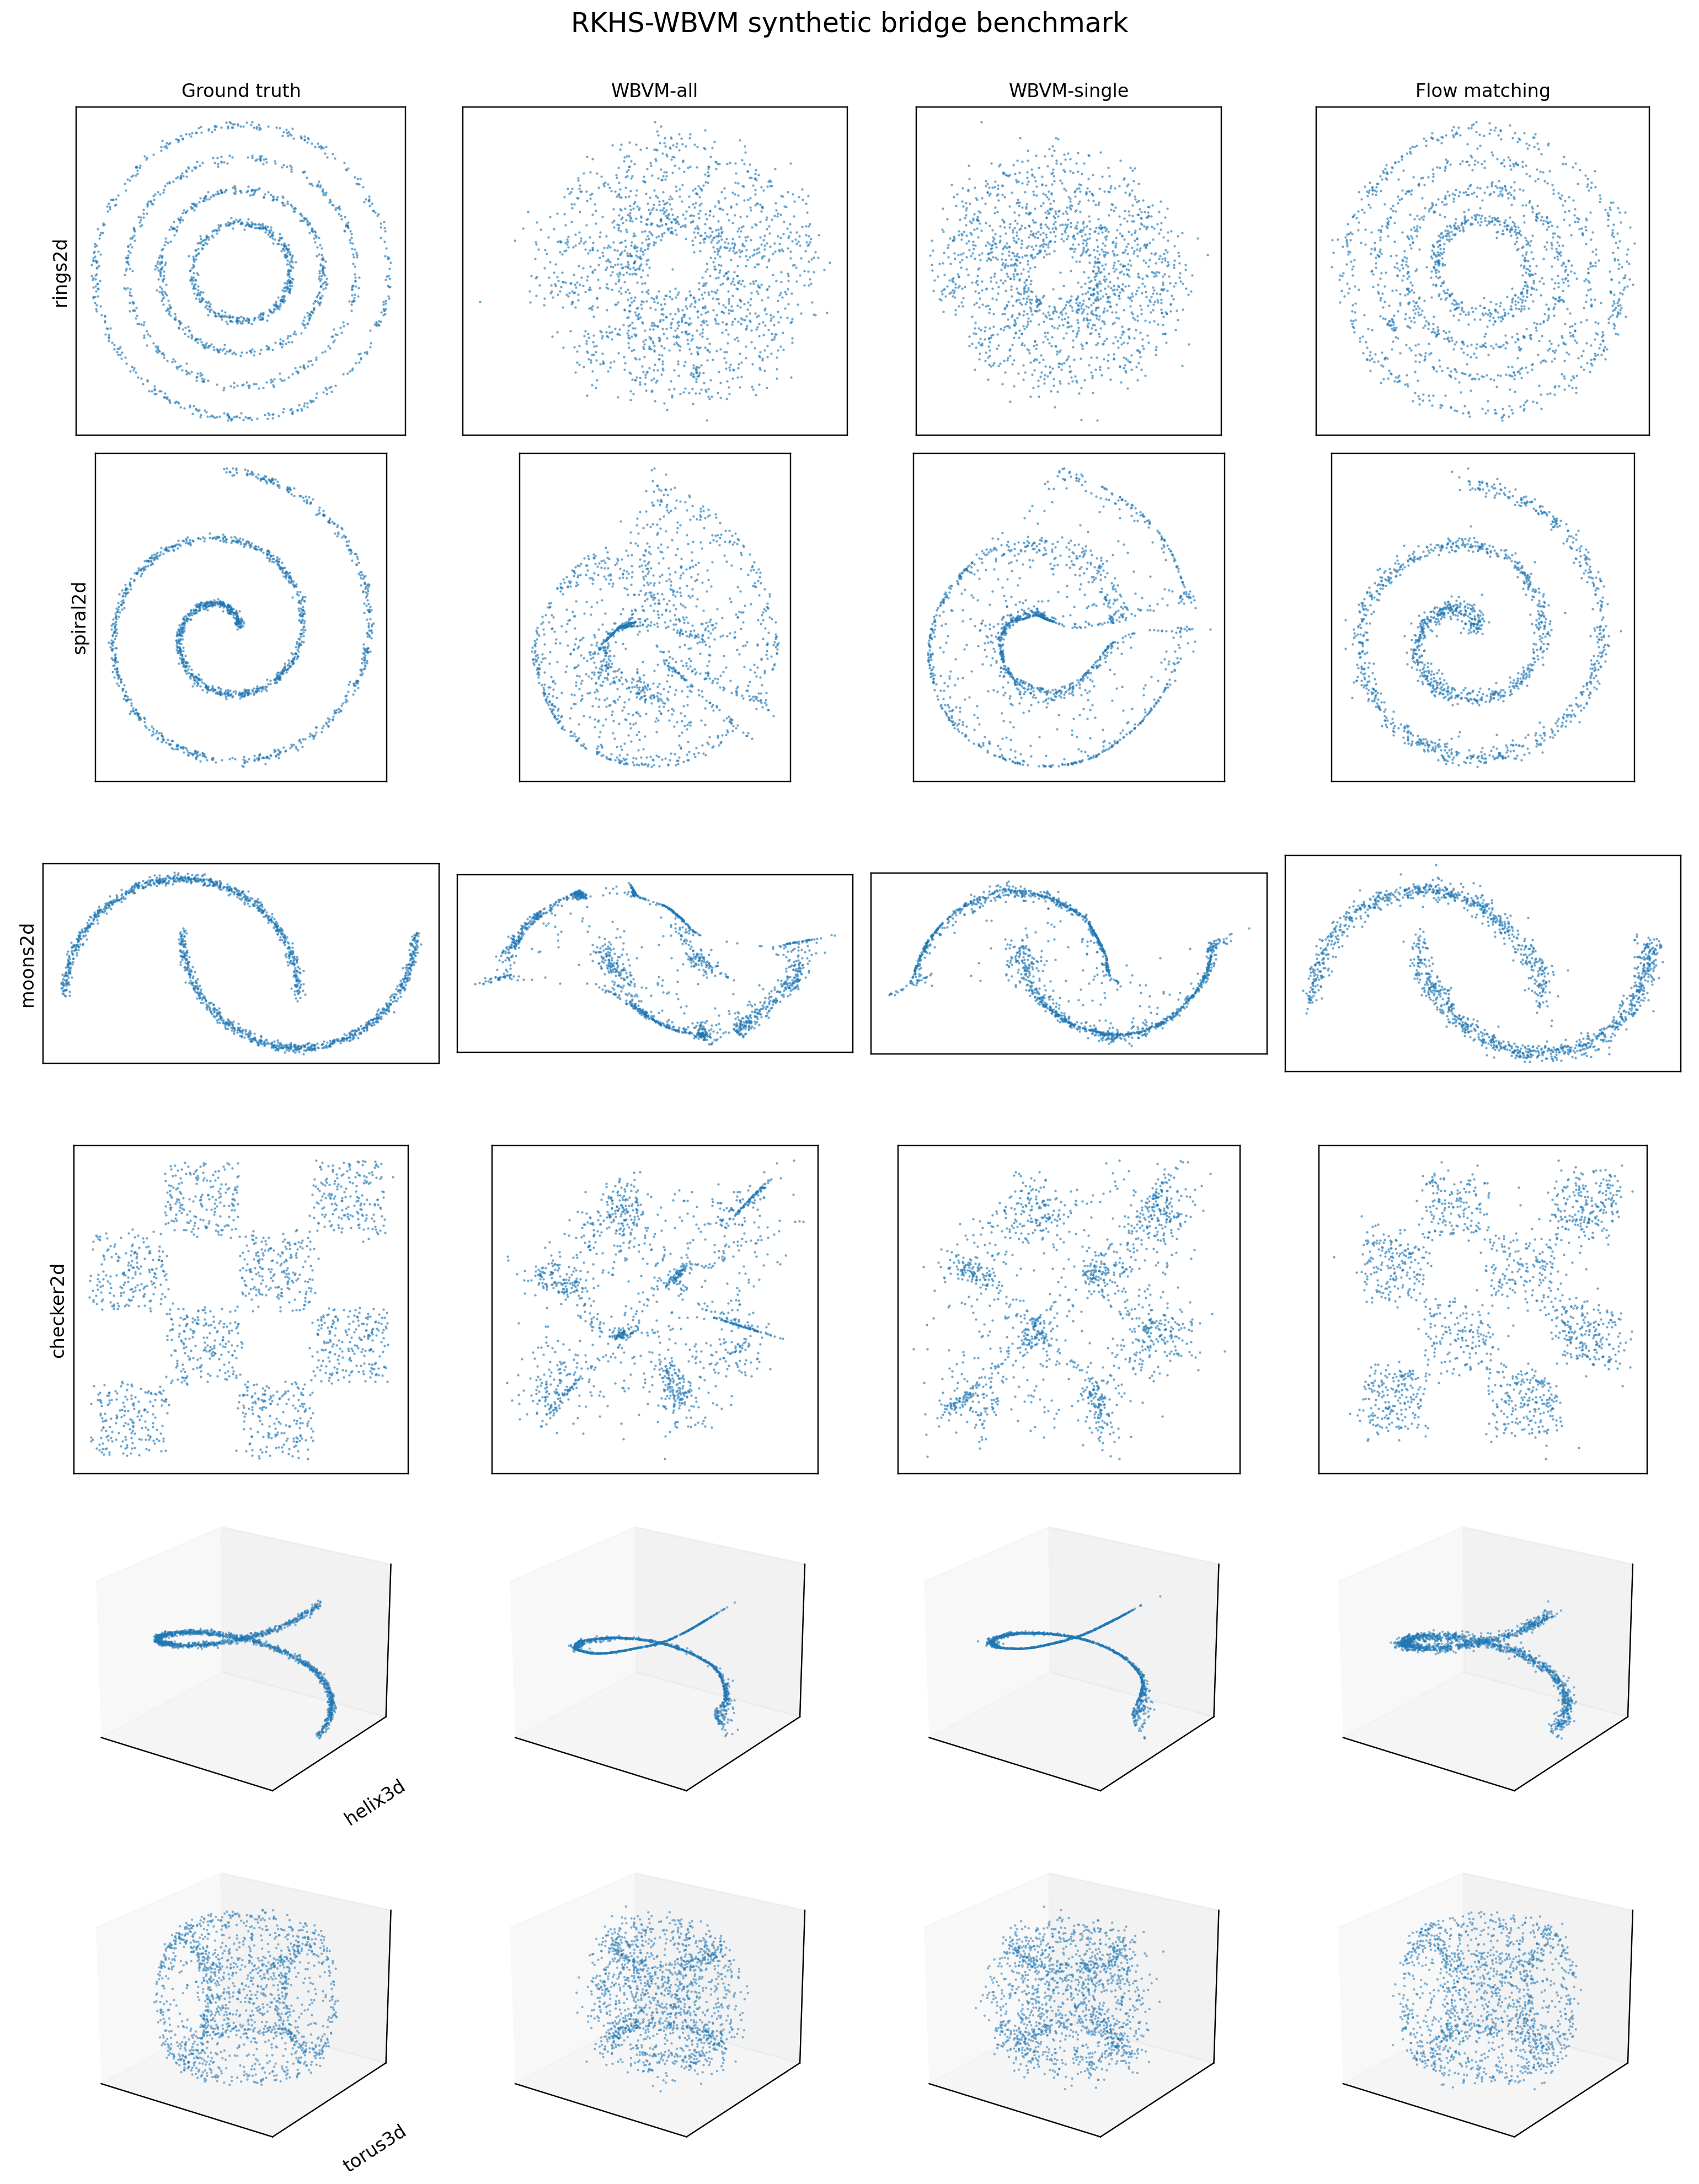
\includegraphics[width=\linewidth]{figures/rkhs_wbvm_toy_6x4_improved.png}
\caption{RKHS-WBVM 稳定化版本在六个 toy 数据集上的生成结果。列依次为 ground truth、WBVM-all、validation-selected WBVM-single 和 flow matching。}
\end{figure}

\begin{table}[htbp]
\centering
\scriptsize
\caption{Table 1-style synthetic metrics on Section 6.1 toy manifolds. The table merges route-one derivative-kernel RKHS-WBVM, route-two vector-flux MMD-WBVM and the flow matching baseline.}
\resizebox{\linewidth}{!}{
\begin{tabular}{lllrrrrr}
\toprule
Dataset & Method & \(\tau\) / range & NFE & \(W_2\) & Sliced \(W_2\) & \% out & Time/10k (s) \\
\midrule
rings2d & RKHS-WBVM-all & [0.35,0.85] & 1 & 0.2909 & 0.0567 & 34.58 & 0.0005 \\
rings2d & RKHS-WBVM-single & 0.80 & 1 & 0.2873 & \textbf{0.0385} & 33.65 & \textbf{0.0004} \\
rings2d & vMMD-WBVM-all & [0.35,0.85] & 1 & 0.3172 & 0.0725 & 37.11 & 0.0005 \\
rings2d & vMMD-WBVM-single & 0.80 & 1 & 0.2910 & 0.0507 & 38.62 & \textbf{0.0004} \\
rings2d & Flow matching & [0.05,0.95] & 20 & \textbf{0.2781} & 0.0411 & \textbf{23.53} & 0.0110 \\
spiral2d & RKHS-WBVM-all & [0.35,0.85] & 1 & 0.2754 & 0.0695 & 51.48 & 0.0005 \\
spiral2d & RKHS-WBVM-single & 0.90 & 1 & 0.2546 & \textbf{0.0348} & \textbf{19.66} & \textbf{0.0004} \\
spiral2d & vMMD-WBVM-all & [0.35,0.85] & 1 & 0.2923 & 0.0795 & 67.83 & 0.0005 \\
spiral2d & vMMD-WBVM-single & 0.80 & 1 & 0.2887 & 0.0613 & 63.82 & \textbf{0.0004} \\
spiral2d & Flow matching & [0.05,0.95] & 20 & \textbf{0.2535} & 0.0427 & 29.81 & 0.0109 \\
moons2d & RKHS-WBVM-all & [0.35,0.85] & 1 & \textbf{0.2286} & 0.0510 & 14.70 & 0.0005 \\
moons2d & RKHS-WBVM-single & 0.90 & 1 & 0.2394 & \textbf{0.0371} & \textbf{8.37} & \textbf{0.0004} \\
moons2d & vMMD-WBVM-all & [0.35,0.85] & 1 & 0.2668 & 0.0730 & 38.75 & 0.0005 \\
moons2d & vMMD-WBVM-single & 0.90 & 1 & 0.2842 & 0.0609 & 35.96 & \textbf{0.0004} \\
moons2d & Flow matching & [0.05,0.95] & 20 & 0.2361 & 0.0666 & 32.45 & 0.0109 \\
checker2d & RKHS-WBVM-all & [0.35,0.85] & 1 & \textbf{0.2153} & 0.0290 & 6.09 & 0.0005 \\
checker2d & RKHS-WBVM-single & 0.80 & 1 & 0.2498 & \textbf{0.0219} & 6.02 & \textbf{0.0004} \\
checker2d & vMMD-WBVM-all & [0.35,0.85] & 1 & 0.2385 & 0.0501 & 2.70 & \textbf{0.0004} \\
checker2d & vMMD-WBVM-single & 0.80 & 1 & 0.2504 & 0.0368 & 6.35 & \textbf{0.0004} \\
checker2d & Flow matching & [0.05,0.95] & 20 & 0.2247 & 0.0394 & \textbf{0.71} & 0.0109 \\
helix3d & RKHS-WBVM-all & [0.35,0.85] & 1 & \textbf{0.2958} & \textbf{0.0332} & 5.82 & 0.0005 \\
helix3d & RKHS-WBVM-single & 0.70 & 1 & 0.3013 & 0.0343 & \textbf{4.78} & \textbf{0.0004} \\
helix3d & vMMD-WBVM-all & [0.35,0.85] & 1 & 0.3435 & 0.0627 & 24.88 & 0.0005 \\
helix3d & vMMD-WBVM-single & 0.80 & 1 & 0.3159 & 0.0731 & 40.81 & \textbf{0.0004} \\
helix3d & Flow matching & [0.05,0.95] & 20 & 0.3299 & 0.0497 & 39.61 & 0.0109 \\
torus3d & RKHS-WBVM-all & [0.35,0.85] & 1 & 0.3710 & 0.0334 & 29.64 & \textbf{0.0004} \\
torus3d & RKHS-WBVM-single & 0.90 & 1 & 0.3616 & \textbf{0.0286} & 30.64 & \textbf{0.0004} \\
torus3d & vMMD-WBVM-all & [0.35,0.85] & 1 & 1.0735 & 0.6124 & 100.00 & 0.0005 \\
torus3d & vMMD-WBVM-single & 0.60 & 1 & 0.4237 & 0.0783 & 39.58 & \textbf{0.0004} \\
torus3d & Flow matching & [0.05,0.95] & 20 & \textbf{0.3519} & 0.0525 & \textbf{18.61} & 0.0109 \\
\bottomrule
\end{tabular}
}
\end{table}

\clearpage

从表格看，RKHS-WBVM-single 在六个 toy 数据集上的 sliced \(W_2\)
均低于 flow matching；RKHS-WBVM-all 在 moons、checker、helix 和 torus
上也低于 flow matching。路线二 vMMD-WBVM 的计算代价同样低，但在
rings、spiral、moons、helix 和 torus 上的 sliced \(W_2\) 与 off-manifold
比例整体更高；特别是 torus3d 的 vMMD-WBVM-all 出现明显退化。这说明
vector-flux MMD 可以作为一条可训练的路线二比较项，但它并不等同于标量弱连续性
方程残差，且会对弱形式中不可见的向量流差异更敏感。因此当前结论应表述为：
U-statistic、velocity normalization、common \(X_0\) 和多尺度带宽显著改善
了 RKHS 路线的有限样本稳定性，但 pure weak flux 仍可能需要
endpoint/marginal stabilization 才能完全消除 off-manifold 伪解。

\subsection{MNIST-FID endpoint results}

To complement the toy experiments, we also evaluate endpoint sample quality on
MNIST using the MNIST-FID protocol.  Lower values are better.  Table
\ref{tab:mnist-fid-results} reports the corrected pixel-CNN setting and the v3
pixel-DIT setting with the route-two RKHS residual included as an additional
method.

\begin{center}
\refstepcounter{table}\label{tab:mnist-fid-results}
{\small \tablename~\thetable: MNIST-FID endpoint quality for the MNIST experiments. Lower is better.\par}
\vspace{0.6em}
{\small
\begin{minipage}{0.47\linewidth}
\centering
\textbf{Pixel-CNN}\\[0.3em]
\begin{tabular}{lr}
\toprule
Method & MNIST-FID \\
\midrule
Drifting & \textbf{0.424} \\
WBVM-single & 1.973 \\
MeanFlow & 2.267 \\
WBVM-all & 2.417 \\
vMMD-WBVM & 4.422 \\
ShortcutFlow & 34.122 \\
\bottomrule
\end{tabular}
\end{minipage}
\hfill
\begin{minipage}{0.47\linewidth}
\centering
\textbf{v3 Pixel-DIT}\\[0.3em]
\begin{tabular}{lr}
\toprule
Method & MNIST-FID \\
\midrule
Drifting & \textbf{1.497} \\
MeanFlow & 1.686 \\
ShortcutFlow & 4.569 \\
WBVM-single & 6.555 \\
WBVM-all & 7.735 \\
vMMD-WBVM & 10.117 \\
\bottomrule
\end{tabular}
\end{minipage}
}
\end{center}

\clearpage

\section{当前模拟实现中的稳定化细节}

RKHS U-statistic 是实际训练版本的核心，但有限 batch 下仍然容易出现速度范数捷径、星形射线和中心坍缩。当前实验版因此采用四个实现约束。

第一，进入 RKHS flux loss 之前，对模型速度和数据速度分别做 batch RMS 归一化：
\[
\widetilde V^\theta
=
\frac{V^\theta}{
\operatorname{sg}\!\left(
\sqrt{\E_{\rm batch}\|V^\theta\|^2}+\delta
\right)},
\qquad
\widetilde V^d
=
\frac{V^d}{
\operatorname{sg}\!\left(
\sqrt{\E_{\rm batch}\|V^d\|^2}+\delta
\right)}.
\]
其中 \(\operatorname{sg}(\cdot)\) 表示 stop-gradient，实验中取 \(\delta=10^{-6}\)。训练时把
\((V^\theta,V^d)\) 替换成 \((\widetilde V^\theta,\widetilde V^d)\)，从而减少
\(\|v\|^2/\sigma^2\) 对目标的支配。

第二，模型桥和数据桥共享同一个 base noise：
\[
X_{\theta,\tau}=(1-\tau)X_0+\tau h_\theta(U),
\qquad
X^d_\tau=(1-\tau)X_0+\tau X_1 .
\]
这不会改变 population 目标，但在有限 batch 中把比较变成 paired bridge comparison，
显著降低两组独立 base noise 带来的方差。

第三，RBF 带宽不再由当前模型样本动态估计，而是只从真实数据桥
\[
X^d_\tau=(1-\tau)X_0+\tau X_1
\]
预先估计 \(\sigma_0\)。训练使用多尺度核平均
\[
\sigma\in \sigma_0\cdot\{0.5,1,2,4\}.
\]
这样小带宽负责局部流形结构，大带宽负责全局错位，且 loss 尺度不再随生成器早期坏样本漂移。

第四，all-time WBVM 不再使用端点附近过宽的 \([0,1]\) 或 \([0.05,0.95]\) 采样，而是采用
\[
\tau\sim{\rm Unif}[0.35,0.85].
\]
这个区间去掉了 base-noise 主导的小 \(\tau\) 和 kernel Hessian 过尖的大 \(\tau\)。
validation-selected single-level WBVM 仍使用候选集合
\[
\mathcal T=\{0.1,0.2,\ldots,0.9\},
\]
并在 endpoint validation 上选择最终候选。

纯 flux 目标为
\[
\cL_{\rm RKHS\text{-}WBVM}^{\rm pure}
=
D_{\rm RKHS\text{-}flux}^2(\theta,\tau).
\]

讲述时的重点是：这是最干净的 posterior-free 版本；它既有核二样本检验的统计解释，又直接对应弱形式流量差异。

\section{参考文献与链接}

\begin{itemize}[leftmargin=2em]
\item MAGT, \href{https://arxiv.org/abs/2602.19600}{Manifold-Aligned Generative Transport}, 2026.
\item Lipman et al., \href{https://arxiv.org/abs/2210.02747}{Flow Matching for Generative Modeling}, 2022.
\item Albergo, Boffi, Vanden-Eijnden, \href{https://arxiv.org/abs/2303.08797}{Stochastic Interpolants: A Unifying Framework for Flows and Diffusions}, 2023.
\item Gretton et al., \href{https://arxiv.org/abs/0805.2368}{A Kernel Method for the Two-Sample Problem}, 2008 / JMLR version.
\item Li et al., \href{https://arxiv.org/abs/1705.08584}{MMD GAN: Towards Deeper Understanding of Moment Matching Network}, 2017.
\item Mroueh et al., \href{https://arxiv.org/abs/1711.04894}{Sobolev GAN}, 2017.
\end{itemize}

\end{document}
